%The previous two chapters described the background for RL and DL. In this chapter, we will see 
%how these two fields are combined in powerful state-of-the-art algorithms for solving complex reinforcement learning problems.
%In this work, we use all the algorithms presented in this chapter.

The previous chapter described a summarized background for RL concepts and classical algorithms. This chapter aims to go more deeper towards the techniques we are actually going to use in this work. First, we must build the background for Neural Networks (NN) and Multi Layer Perceptrons (MLP), which are commonly used as policy and value function approximations in modern RL algorithms. Then, we will present two state of the art RL techniques which we plan to use in our problem.

\section{Neural Networks}

Neural Networks are mathematical structures that receive inputs and calculate outputs. In this sense, can be described as a mathematical fitter to very complex and non-linear functions.

Also known as Multi Layer Perceptron (MLP), it has a multiple layer architecture, where each layer is composed by several nodes called neurons. These nodes, in an analogy to human brain neurons, are still mathematical units which receives some numerical inputs and outputs one single number. All of these mathematical units make use of a specific set of parameters.

\subsection{Representation}

Regarding the representations and notations used for NN, we can describe its basic elements consisting of inputs, outputs, parameters and activate functions.

For each one of the $m$ training examples, we define the input $x^(i)$, corresponding to the $i$ example, as a n-dimensional feature column vector, so with dimensions $(n,1)$. It is also called the input layer, with index $0$, and also represented as $a^{[0](i)}$ with dimensions $(n^{[0]},1)$.

For each layer $l$, also called hidden-layers, with $1<l<L$ in a total of $L$ layers, we have a specific structure:
\begin{itemize}

\item
	The layer $l$ has a total of $n^{[l]}$ hidden units, each $j$th unit receives all the inputs $a^{[l-1](i)}$ from layer $l-1$, and output a scalar $a^{[l](i)}_j$. The total output of the layer is then composed by all hidden units outputs, given by the vector $a^{[l](i)}$, with dimensions $(n^{[l]},1)$.
	
\item
	Each $j$th hidden unit has a row-vector linear parameter $w^{[l]}_j$ with dimensions $(1,n^{[l-1]})$. The total linear parameters $w^{[l]}$ of the layer is given by all hidden units parameters in a $(n^{[l]},n^{[l-1]})$ matrix.
	
\item
	Each $j$th hidden unit also has a scalar bias-parameter given by $b^{[l]}_j$, and all units bias-parameters compose the layer bias vector $b^{[l]}$, with dimensions $(n^{[l]},1)$
	
\item
	The layer also has a specific activation function $g^{[l]}(z)$, which can assume different mathematical functions, such as the \textit{sigmoid} function, the \textit{tanh} function, and, the most common, the \textit{ReLU} function, shown in equation \ref{eq:common_activation_functions}.

\begin{equation}
sigmoid(z) = \frac{1}{1+e^{-z}} \text{ ; } tanh(z) = \frac{e^z - e^{-z}}{e^z + e^{-z}} \text{ ; } Relu(z) = max(z,0)
\label{eq:common_activation_functions}
\end{equation}

\end{itemize}

All these elements of the layer are related through the update equations \ref{eq:linear_update_nn} and \ref{eq:non_linear_update_nn}, which, for each layer $l$, receives the previous layer output $a^{[l-1]}$ and generates the current layer output $a^{[l]}$. The figure \ref{fig:nn_basic_architecture} illustrates this representation for a shallow one hidden-layer NN.

\begin{align}
z^{[l](i)} = w^{[l]}a^{[l-1](i)} + b^{[l]}
\label{eq:linear_update_nn}
\\
a^{[l](i)} = g^{[l]}(z)
\label{eq:non_linear_update_nn}
\end{align}

\begin{figure}[H]
    \centering
    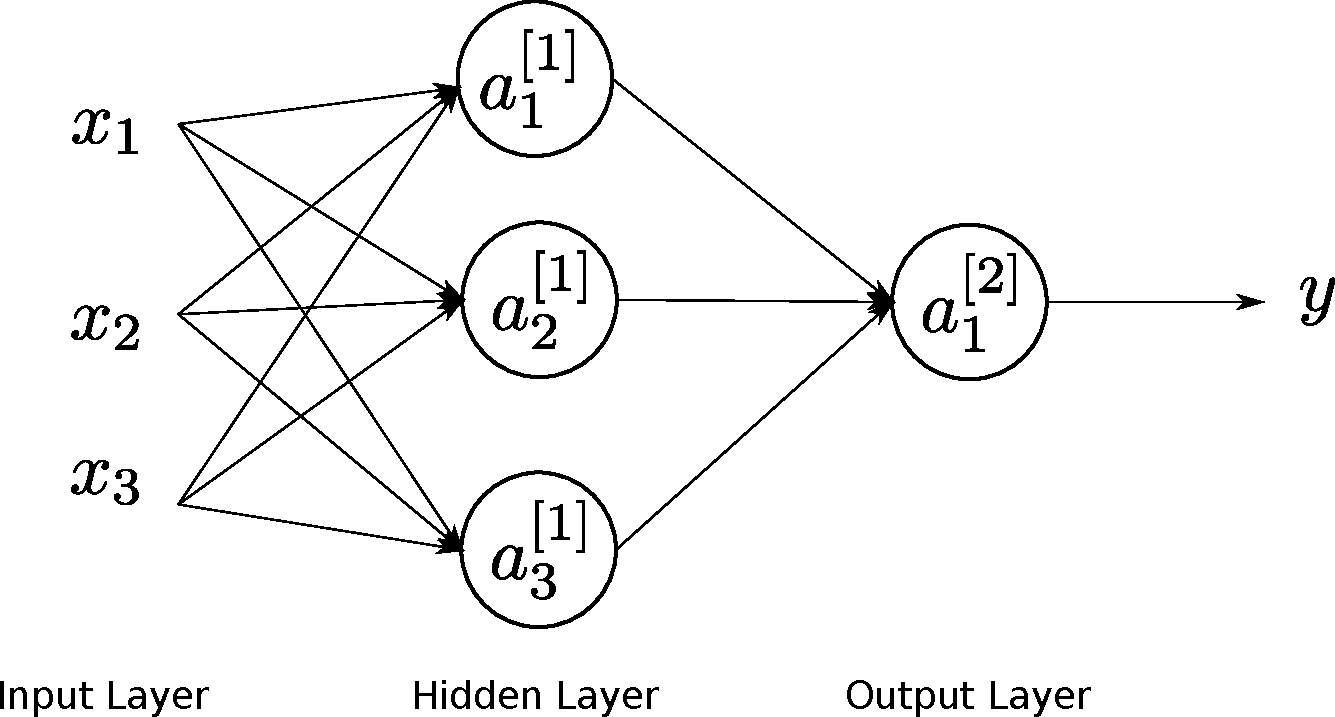
\includegraphics[width=0.6\textwidth]{Chapter4/neuralnet.pdf}
    \caption{Shallow Neural Network Architecture}
    \label{fig:nn_basic_architecture}
\end{figure}

% describe:
% para cada exemplo de 1 a m, temos um vetor de input x (n[0],1)
% para cada camada de 1 a L, temos:
%			 n[l] hidden units,
%			 uma matriz de parametros W (n[l],n[l-1])
%			 e um vetor de bias b (n[l],1)
% activation functions
% cost function

\subsection{Vectorization}

The previous equations are capable of fully defining update rules for any MLP, however, in order to avoid the naively computation over each training example, and therefore reach more efficient algorithms exploring the use of parallelization in modern GPUs architectures, we must introduce a vectorization notion.

Let's first define the $X$ matrix as the concatenation of each training example $x^{(i)}$ composing its columns, in a way that:

\begin{equation*}
X = \left[ x^{(1)}, x^{(2)}, ..., x^{(m)} \right]
\end{equation*}

\subsection{Forward Propagation}

\subsection{Backward Propagation}

\subsection{Optimizations}

\section{Trust Region Policy Optimization}


\section{Proximal Policy Optimization (PPO)}
